\documentclass[11pt,twocolumn,final]{article}
\usepackage{verbatim}
\usepackage[final]{pdfpages}
\usepackage{biblatex}
\usepackage{float}
\bibliography{mybib}

\begin{document}
\onecolumn
%filename, caption, width in mm
\newcommand{\newfigure}[4]{
	\begin{figure}[#4]
	\begin{center}
	\includegraphics[#3]{figures/#1.png}
	\caption{#2}
	\label{fig:#1}
	\end{center}
	\addtocontents{lof}{\vskip 1.0em}
	\end{figure}
}

\newcommand{\spacesubsection}[1]{
	\subsection{#1}
	\addtocontents{toc}{\vskip 1.0em}
}
%%%%% Title Page %%%%%%
\title{Multi-File Code Coverage in DrRacket}
\author{Jonathan Walsh}
\date{\vfill
Computer Science Department \\
College of Engineering \\
California Polytechnic State University \\
2011\\[8mm]
\begin{flushright}
Submitted: \today\\
Advisor: John Clements
\end{flushright}}
\maketitle
\thispagestyle{empty}
\newpage

%-------------------- Front Matter --------------------%

%%%%% Table of Contents %%%%%
\renewcommand{\thesubsection}{\Roman{subsection}}
\renewcommand{\thesubsubsection}{\arabic{subsection}}
\pagenumbering{roman} 
\tableofcontents 
\newpage

%%%%% Abstract %%%%%
\addcontentsline{toc}{section}{\textnormal{Abstract}}
\section*{Abstract}
Lorem ipsum dolor sit amet, consectetur adipiscing elit. 
\newpage

%%%%% List of Figures %%%%%
%\addcontentsline{toc}{section}{\textnormal{List Of Figures}}
%\listoffigures
%\newpage

%figures
%\newfigure{covered-files-dialog}{Covered Files Dialog}{width=8.5cm}
%\newfigure{uncovered-lines-dialog}{Uncovered Lines Dialog}{width=6cm}
%\newfigure{no-coverage-found-dialog}{No Coverage Found Dialog}{width=10cm}
%\newfigure{out-of-date-dialog}{Out Of Date Dialog}{width=10cm}
%\newfigure{coverage-button}{Multi-File Coverage Button in DrRacket}{width=12cm}
%\newfigure{default-flow}{Example DrRacket Code Coloring}{width=7.5cm}
%\newfigure{extended-flow}{Example DrRacket Code Coloring}{width=11cm}

%-------------------- Report --------------------%
%\twocolumn
\pagenumbering{arabic} 
\addtocontents{toc}{\contentsline {section}{\normalfont{\textit{Section}}}{}}

%%%%% Intro %%%%%
\spacesubsection{Introduction}
Lorem ipsum dolor sit amet, consectetur adipiscing elit. 

\newfigure{covered-files-dialog}{Covered Files Dialog}{width=8.5cm}
\newfigure{uncovered-lines-dialog}{Uncovered Lines Dialog}{width=6cm}
\newfigure{no-coverage-found-dialog}{No Coverage Found Dialog}{width=10cm}
\newfigure{out-of-date-dialog}{Out Of Date Dialog}{width=10cm}
\newfigure{coverage-button}{Multi-File Coverage Button in DrRacket}{width=12cm}

%%%%% Background %%%%%
\spacesubsection{Background}
\label{background}
Racket is a programming language \cite{racket}. Included with every download of Racket is an integrated development environment (IDE), DrRacket. DrRacket is the ``official'' IDE for Racket and is maintained by the same core group of contributors. 

\newfigure{drracket}{DrRacket}{width=10.5cm}{h!}

DrRacket's user interface is divided into two main areas: the definitions window, by default on top, and the interactions window. The definitions window contains the source file while the interactions window displays the program's output. Above the definitions window are a horizontal list of buttons. Included in this list is the ``run'' button, which, when pressed, executes the program in the definitions window. See figure \ref{fig:drracket} for a sample DrRacket environment.

DrRacket's default code coverage can be enabled by selecting ``Syntactic Test Suite Coverage'' in the ``Choose Language'' dialog. Once code coverage has been enabled, it is collected every time the program is executed by clicking the ``run'' button. The code coverage information is then displayed by coloring covered code green and uncovered code red. (Figure~\ref{fig:drracket}). However, if the entire program is covered, in which case no code coloring is done.

In order to determine which sections of code to color, DrRacket must keep track of which expressions of have been executed. DrRacket does this by adding additional code, hidden from the user, before the program is run. This added code surrounds every expression with an integer variable that represents the number of times the expression has been executed. So, if the variable is 0 the expression has not been executed. Then, by examining these variables, it can be determined which sections of code have not been executed. Additionally, these variables can be used to profile which sections of code are heavily used, but is not the focus of this senior project and will not be covered. Figure \ref{fig:default-flow} shows the simplified program flow for code coverage and code highlighting in DrRacket before the solution implemented by this senior project.

\newfigure{default-flow}{DrRacket Code Coverage Flow}{width=7cm}{h!}

DrRacket can be extended in two ways, either through a new collection or a PLaneT package. Collections are tightly coupled with DrRacket and are often distributed with the default installation. PLaneT packages, on the other hand, are more modular. They can be downloaded and automatically installed form a central package repository. Both methods can be used to create new tools for DrRacket. At start up DrRacket looks for tools by reading \emph{info.rkt} files found in collections and installed PLanT packages \cite{plugin}. These tools can then extend DrRacket through the use of mixins. Every major component of DrRacket is a mixin, from the ``Run'' button to tabs. 


%%%%% Research %%%%%
\spacesubsection{Research}
Before attempting to implement a solution to extend DrRacket's code coverage to multiple files, research was required to better understand how DrRacket implements and uses code coverage. This research consisted primarily of modifying small sections of DrRacket and then examining the results. While this process was not particularly fast, it did eventually reveal the information needed to successfully implement the tool.

During the research, the following facts where discovered: one, the organization of DrRacket's user interface follows the hierarchy seen in figure \ref{fig:gui-classes}; two, DrRacket generates a test coverage info hash table that contains information for all uncompiled required files; and three, the test info hash table persists after code coloring has been applied.

DrRacket's user interface is composed of four main classes, seen as boxes in figure \ref{gui-classes}. The highest class is the \emph{frame}. The \emph{frame} is an entire DrRacket environment as seen in figure \ref{fig:drracket}. Each frame has at least one \emph{tab}. A \emph{tab} always contains a definitions window, where the source code is visible and editable. A \emph{tab} may also contain an interactions window. Additionally, the frame group contains a list of all currently open \emph{frames}.

\newfigure{gui-classes}{DrRacket User Interface Classes}{width=6cm}{h!} 

%add detail about testing methods
DrRacket generates a hash table, called \emph{test-coverage-info} internally, when the program is run. Included in the hash table are expressions, with their respective source code location, and whether or not they have been evaluated. By examining the contents of the test coverage info hash table, for a program that includes multiple files, it was discovered that coverage information is collected for all uncompiled files. So while DrRacket's default code coverage only applies code coloring to the active file, the test coverage info hash table has the information needed to color additional files. Code coverage can not be collected for compiled files because their code can not be expanded to track executed expressions, see figure \ref{fig:default-flow}.

The test coverage info hash table can be sent to a method of DrRacket's \emph{tab} class, called \emph{show-test-coverage-annotations}, which does code coloring for that tab based on the hash table. This hash remains available for use after code coloring has been completed. In order to clear the test coverage info hash table an additional method, \emph{clear-test-coverage}, must be called. 



%%%%% Implementation %%%%%
\spacesubsection{Implementation}
The Multi-file Code Coverage Tool is implemented as a PLaneT package. This requires no modification to any of DrRacket's source files and satisfies one of the additional goals for the project. PlaneT also brings the benefits of easy distribution, installation, updating, and feedback for the tool. The Multi-file Code Coverage Tool works in the following steps: first, searching for a test info hash table; second, coloring the code of currently open files; and third, displaying a series of dialogs that give the user test coverage information. This process can be seen in figure \ref{fig:extended-flow} on page \pageref{fig:extended-flow}.

The Multi-file Code Coverage Tool adds a new button to DrRacket, labeled ``Multi-file Coverage'' (Figure \ref{fig:coverage-button}). Clicking this button will color code in all open tabs using the currently in focus tab's test coverage info hash table. This means, if the user opens their test program and runs it and then clicks the button, all open tabs will be colored relative to the test file. However, if the user switches to another file, before clicking the ``Multi-file Coverage'' button, the newly switched to file's test coverage info will be applied. This behavior, while perhaps not immediately obvious, allows for code coverage information and highlighting to be quickly switched between.

\newfigure{coverage-button}{Multi-File Coverage Button in DrRacket}{width=9cm}{h!}

\newfigure{extended-flow}{Extended DrRacket Code Coverage Flow}{width=10cm}{h!}

After the ``Multi-file Coverage'' button is pressed the first thing done is loading the test coverage info hash table. This hash table contains all the information needed to properly display code coverage. There are two places that the test coverage info hash table may be found: in the current \emph{tab's} memory or as a saved coverage info file. If it is found in memory that means the program was recently run and the hash table is as up to date as it possibly can be. For this reason loading the hash table from memory is preferred. However, if the test coverage info could not be found in memory then it is looked for on the disk. The saved hash table is placed in a ``compiled'' directory next to the source file. This ``compiled'' directory is also where DrRacket would place a compiled versions of the source program. Every program only has one saved coverage file. It's file name is the same of the source file, but with a special coverage extension. When the test coverage info is loaded from a saved file it may be out of date. So, the save file's last modification date is compared to that of the source file's. If the save file was modified more recently than the source file a warning, as seen in figure \ref{fig:out-of-date-dialog}, is displayed. The user may choose to ignore this warning. While doing so means that code coverage will used outdated information, it allows the user to load code coverage information without running the source file again. This could be useful if the source file is large and takes a long time to run. If the test coverage information could not be found, either in memory or in a save file, an error message is displayed, as seen in figure \ref{fig:no-coverage-found-dialog}. Finally, if the test coverage info was loaded from memory, then the data is written to the coverage save file.

\newfigure{out-of-date-dialog}{Out Of Date Dialog}{width=8.5cm}{h!} 
\newfigure{no-coverage-found-dialog}{No Coverage Found Dialog}{width=8.5cm}{h!}


Next the loaded code coverage information is sent to open files that were covered by the source file to do code coloring. Each code expression in the test info coverage hash table has a file name attached to it. So, by searching through the coverage information a list of covered files can be computed. The coverage info is then applied to every open file. A list of open files are found by looking through every \emph{tab}, in every \emph{frame} found in the \emph{frame group}. Then, for each open file, that is also covered by the source file, the test coverage info is sent to it. No reduction of the test coverage has table is needed before applying it to a file, even though it will contain irrelevant coverage information. The \emph{show-test-coverage-annotations} method in \emph{tab} will only use the relevant information. During the process of sending coverage information to tabs, it is also computed if the coverage is valid. Coverage information can become invalid when the file being receiving it has been modified after the coverage information was collected. The test coverage info hash table has no internal way of determining it's validity. So, before it is sent a check is preformed by comparing the last modification date of the saved coverage file and the source file. If the source file has been modified after the source file then its test coverage is considered invalid and no code coloring will be done to it. This information will also appear as an asterisk in the Covered Files Dialog (Figure \ref{fig:covered-files-dialog}). As mentioned in section \ref{background}, background, only uncompiled files are included in the test coverage info hash table. However, this provides more benefits the drawbacks. The largest benefit being that none of DrRacket's source files are included because they are all compiled.

\newfigure{covered-files-dialog}{Covered Files Dialog}{width=7cm}{h!}

The finial step of the Multi-file Code Coverage Tool is displaying a series of dialogs to inform the user on the collected coverage information. The first one displayed is the Covered Files Dialog (Figure \ref{fig:covered-files-dialog}). This displays a list of files that have been covered by the source file. Next to each file is that file's covered line percent. So, 100\% indicates that the entire file is covered. The files are sorted in acending order by covered percent. This is done because it is resonable that the user is more interested in files with uncovered code. The user may then select one, or more, files to switch too focus too, or open if needed, by clicking ``Open''. If the selected files were not already open, the code coveverage hash table is sent to them so that they may apply code coloring. Additionally, the user may selected the ``Open With Uncovered Lines Dialog'' indstead. This button will behavie like the ``Open'' button with the addition of displaying another Uncovered Lines Dialog (Figure \ref{fig:uncovered-lines-dialog}). This displays a list of lines containig uncovered code in the file that was just opened. The list of uncovered lines allows the user to more quickly find lines of interest. Without it the user must visualy scan the entire file for sectons of code that have been colored red.

\newfigure{uncovered-lines-dialog}{Uncovered Lines Dialog}{width=5cm}{h!}

%%%%% Evaluation %%%%%
\spacesubsection{Evaluation}
The evaluation of this senior project was done in two parts: first, an evaluation of the Multi-file Code Coverage Tool; and second, an evaluation of developing it for DrRacket.

The Multi-file Code Coverage tool successfully extends DrRacket's code coverage to multiple source files. It does so without requiring any modifications to DrRacket's source code. Additionally, it provides concrete information to the user on the amount of covered code versus uncovered code. These were the main foci of this senior project. The Multi-file Code Coverage tool has been available on PLaneT for, at the time of this writing, approximately two weeks. Thus far, no bugs have been reported.

While the tool meets all of the requirements, it does have a few areas that could be improved upon. First, the detection of valid files does not work in some cases. Specifically, files that have been modified, but not saved, and are not in the focused \emph{tab} of a \emph{frame}, will report that the coverage is valid. Fixing this would require learning more details of the DrRacket user interface and its management. Second, the Multi-file Code Coverage Tool could be slightly better integrated with DrRacket. One possible way of doing this would be extending the ``Run'' button to automatically save coverage information. Currently, if the user runs the program, modifies it, and then attempts to load multi-file coverage, it will load outdated data. By also integrating the tool with the ``Run'' button the most recent test coverage information would always be saved. Finally, the parsing of the test coverage info hash table is not particularly fast, especially on larger projects. Further research could be done to improve the efficiency of the algorithm, cache data, or some other method to speed it up.

Overall, developing the Multi-file Code Coverage Tool for DrRacket went smoothly. DrRacket is well documented and there are many tutorials available on docs.racket-lang.org. However, there were a few issues that were encountered during the development of the tool: one, lower level methods and variables were not as well documented; two, finding new information was sometimes difficult; and three, there were limited external Racket resources. All of the issues presented next may actually have solutions that were not discovered. However, if this is the case then another issue is present: understanding DrRacket is difficult and takes a long time. Each issue presented was exhaustively researched by myself, and if I failed to find the correct answer then better documentation and explanations are needed.

While most high level, and often used, functions are well documented, lower level ones are not as well. This presented challenges when trying to determine what the purpose of the function was. One specific example is the variable called \emph{test-coverage-enabled}. There are actually two separate variables in DrRacket's source, both named \emph{test-coverage-enabled}. One used by DrRacket's user interface and one used by the code coverage generation. Additional documentation could have made this clearer. Overall DrRacket's low level documentation was much better than what I have seen in other projects.

Finding related functions and documentations was not always obvious. One example of this was seen when attempting to find all of the active DrRacket \emph{frames}. I thought I had searched everywhere for a function to find them. It was not until I was pointed to the \emph{group:get-the-frame-group} function that I was able to find the needed functions. No where else had I seen mentions of groups and had no reason to search for them. However, this is not a problem inherent with DrRacket, but one that is present in projects with a large code base.

Finally, since Racket and DrRacket are not as widely used as Java or C++, there were limited external resources on the subject. This presented problems when I would attempt to research, what I felt would be common error messages. Often I would only find one or two results, both on the Racket mailing list. The answers provided there would not always fix my problem. This is in comparison to searching a Java error, where pages of results, that include sites such as Stack Overflow, are displayed. This forced me to ask my advising professor, John Clements, many questions that had simple answers I could have figured out independently had it been a more common language. 

%%%%% Conclustion %%%%%
\spacesubsection{Conclusion}
Lorem ipsum dolor sit amet, consectetur adipiscing elit. 

\newfigure{covered-files-dialog}{Covered Files Dialog}{width=8.5cm}
\newfigure{uncovered-lines-dialog}{Uncovered Lines Dialog}{width=6cm}
\newfigure{no-coverage-found-dialog}{No Coverage Found Dialog}{width=10cm}
\newfigure{out-of-date-dialog}{Out Of Date Dialog}{width=10cm}
\newfigure{coverage-button}{Multi-File Coverage Button in DrRacket}{width=12cm}

%-------------------- Bib --------------------%
\onecolumn
%\bibliographystyle{plain}
%\bibliography{mybib}
\newpage
\addcontentsline{toc}{section}{\textnormal{List Of Figures}}
\listoffigures
\addcontentsline{toc}{section}{\textnormal{References}}
\nocite{*}
\printbibliography

%-------------------- Appendix --------------------%
\newpage
\addtocontents{toc}{\contentsline {section}{\normalfont{\textit{Appendix}}}{}}
\renewcommand{\thesubsection}{\Alph{subsection}}
\appendix

\section*{Appendixes}
%%%% Source Code %%%%
\spacesubsection{Source Code}
\subsubsection*{info.rkt}
\tiny{
\verbatiminput{../info.rkt}
}

\subsubsection*{info-helper.rkt}
\tiny{
\verbatiminput{../info-helper.rkt}
}

\subsubsection*{tool.rkt}
\tiny{
\verbatiminput{../tool.rkt}
}

%%%%% PLaneT Documentation %%%%%
% steps to get it in here:
% 1) generate latex from code-coverage.scrbl
% 2) in the .tex file add \setcounter{page}{<page number>} right after the documentclass
% 3) generate a pdf from the .tex file
\spacesubsection{PLaneT Documentation}
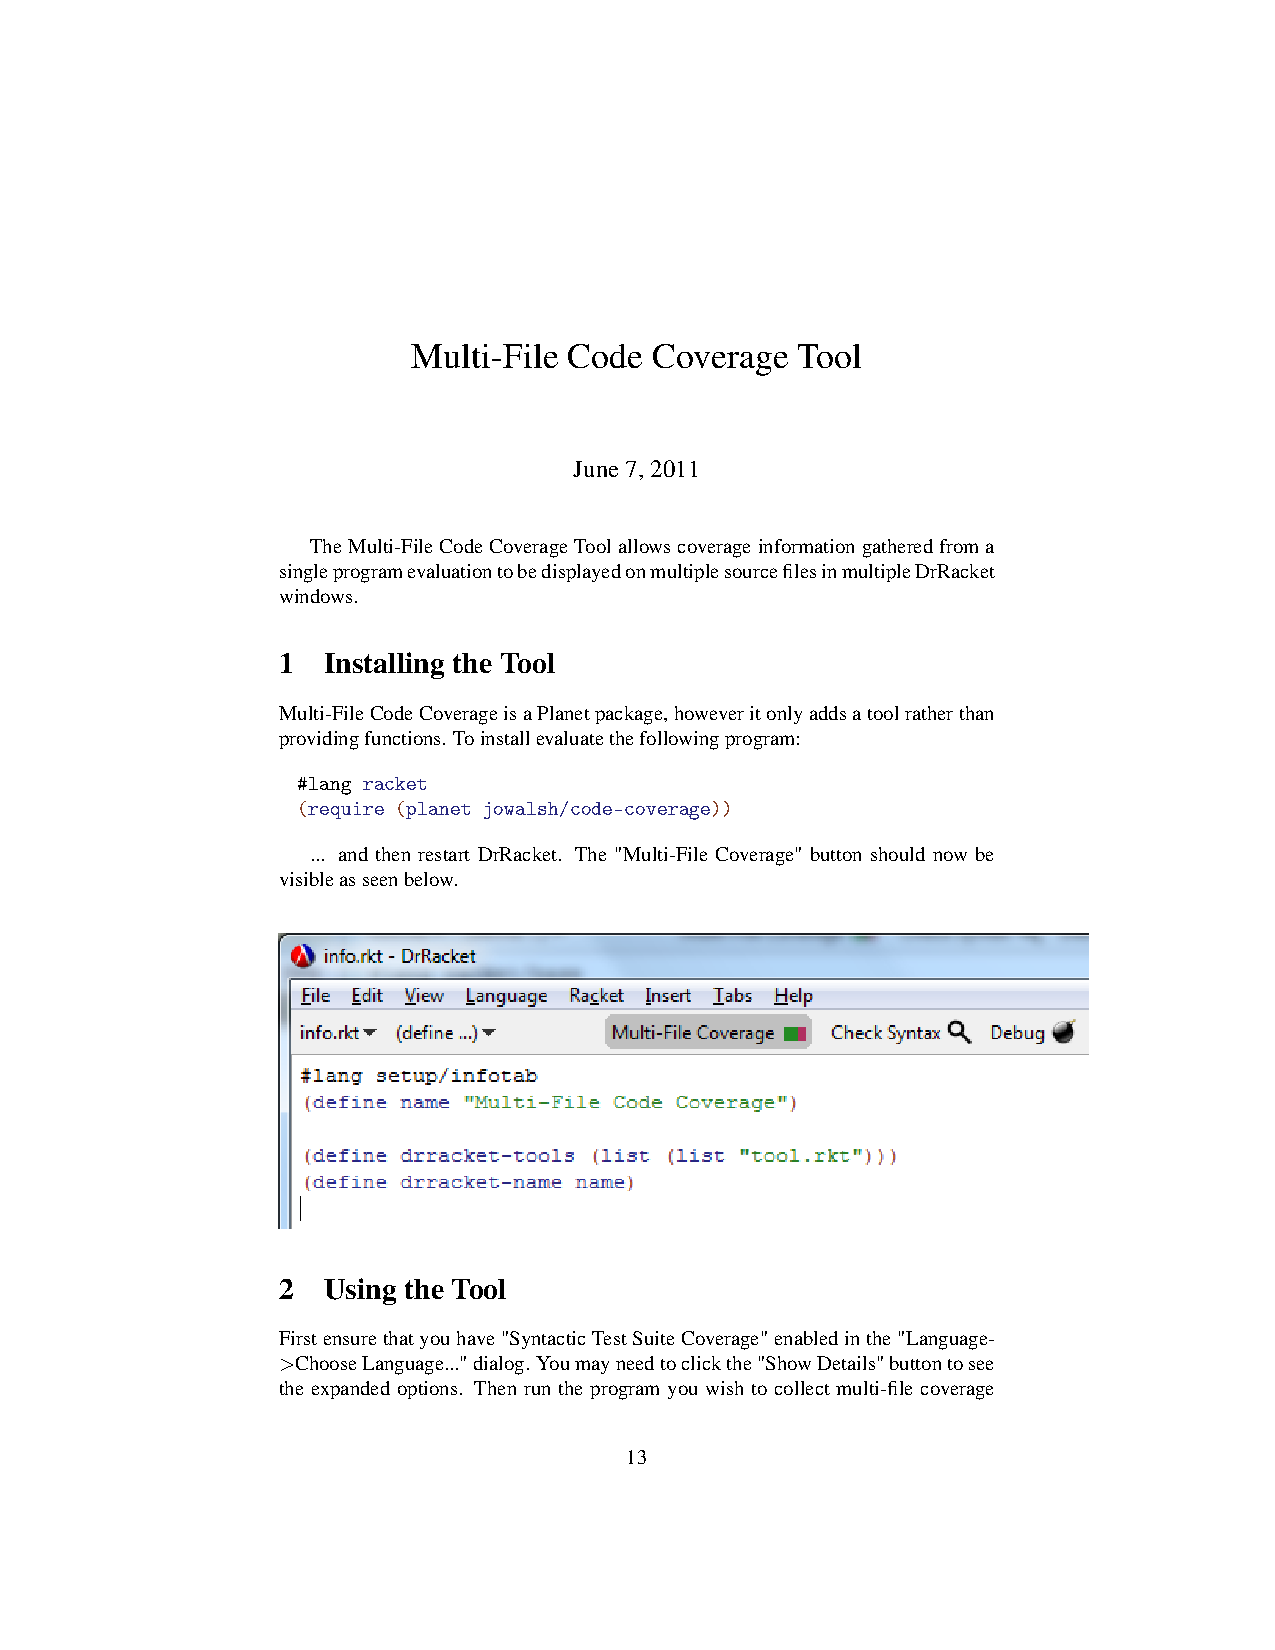
\includepdf[pages=-]{scribble/code-coverage.pdf}

\end{document}
